\chapter[Modelagem Ensemble]{Modelagem Ensemble}

\begin{objetivos}
	Ao final desta unidade, o estudante deverá compreender o conceito de modelagem ensemble em SDM; integrar predições de GLM, GAM, Random Forest, BRT e Maxent; comparar ensemble por média simples, média ponderada e consenso binário; ponderar modelos por desempenho preditivo; gerar mapas de adequabilidade ensemble para \textit{Dinizia excelsa}; avaliar a concordância entre modelos; e preparar produtos para projeções futuras, avaliação de incertezas e aplicações à conservação.
\end{objetivos}

\section{Introdução}

A Modelagem Ensemble é uma abordagem amplamente utilizada em Modelagem de Distribuição de Espécies para combinar predições de diferentes algoritmos. Em vez de depender de um único modelo, o ensemble integra múltiplas representações estatísticas da relação entre ocorrência e ambiente, reduzindo a dependência de escolhas algorítmicas específicas \parencite{araujo2007ensemble,thuiller2009biomod,guisan2017habitat}.

Em SDM, diferentes algoritmos podem produzir mapas distintos porque representam respostas ambientais de maneiras diferentes. GLM e GAM são mais interpretáveis; Random Forest e BRT capturam relações complexas; Maxent é especialmente adequado para dados presença-background. O ensemble sintetiza essas diferenças em um produto integrado.

\begin{conceito}[title={\faBook\quad Ensemble em SDM}]
	Um ensemble combina predições de múltiplos modelos para representar uma estimativa integrada da adequabilidade ambiental. Ele não elimina incertezas, mas permite quantificar concordância e divergência entre algoritmos.
\end{conceito}

\section{Tipos de ensemble}

Nesta unidade serão considerados três tipos principais de ensemble:

\begin{itemize}
	\item média simples das predições;
	\item média ponderada por desempenho preditivo;
	\item consenso binário baseado em limiares de presença-ausência.
\end{itemize}

A média simples considera todos os modelos com o mesmo peso. A média ponderada atribui maior influência aos modelos com melhor desempenho. O consenso binário representa a proporção de modelos que classificam uma célula como adequada.

\begin{atencao}[title={\faExclamationTriangle\quad Ensemble não corrige modelo ruim}]
	O ensemble deve ser construído a partir de modelos minimamente aceitáveis. Incluir modelos com baixa qualidade, forte sobreajuste ou respostas ecologicamente incoerentes pode degradar o resultado final.
\end{atencao}

\section{Preparação das predições}

Nesta unidade, integramos os mapas de adequabilidade gerados nas Unidades 6 a 10. Todos os rasters devem possuir a mesma extensão, resolução, projeção e máscara espacial.

\rscriptfile{scripts/unidade11/01_estrutura_pastas.R}

\rscriptfile{scripts/unidade11/02_preparar_predicoes_ensemble.R}

\section{Ensemble por média simples}

A média simples representa a adequabilidade média prevista pelos modelos. É uma abordagem transparente e útil quando todos os modelos têm desempenho semelhante.

\rscriptfile{scripts/unidade11/03_ensemble_media_simples.R}

\begin{figure}[H]
	\centering
	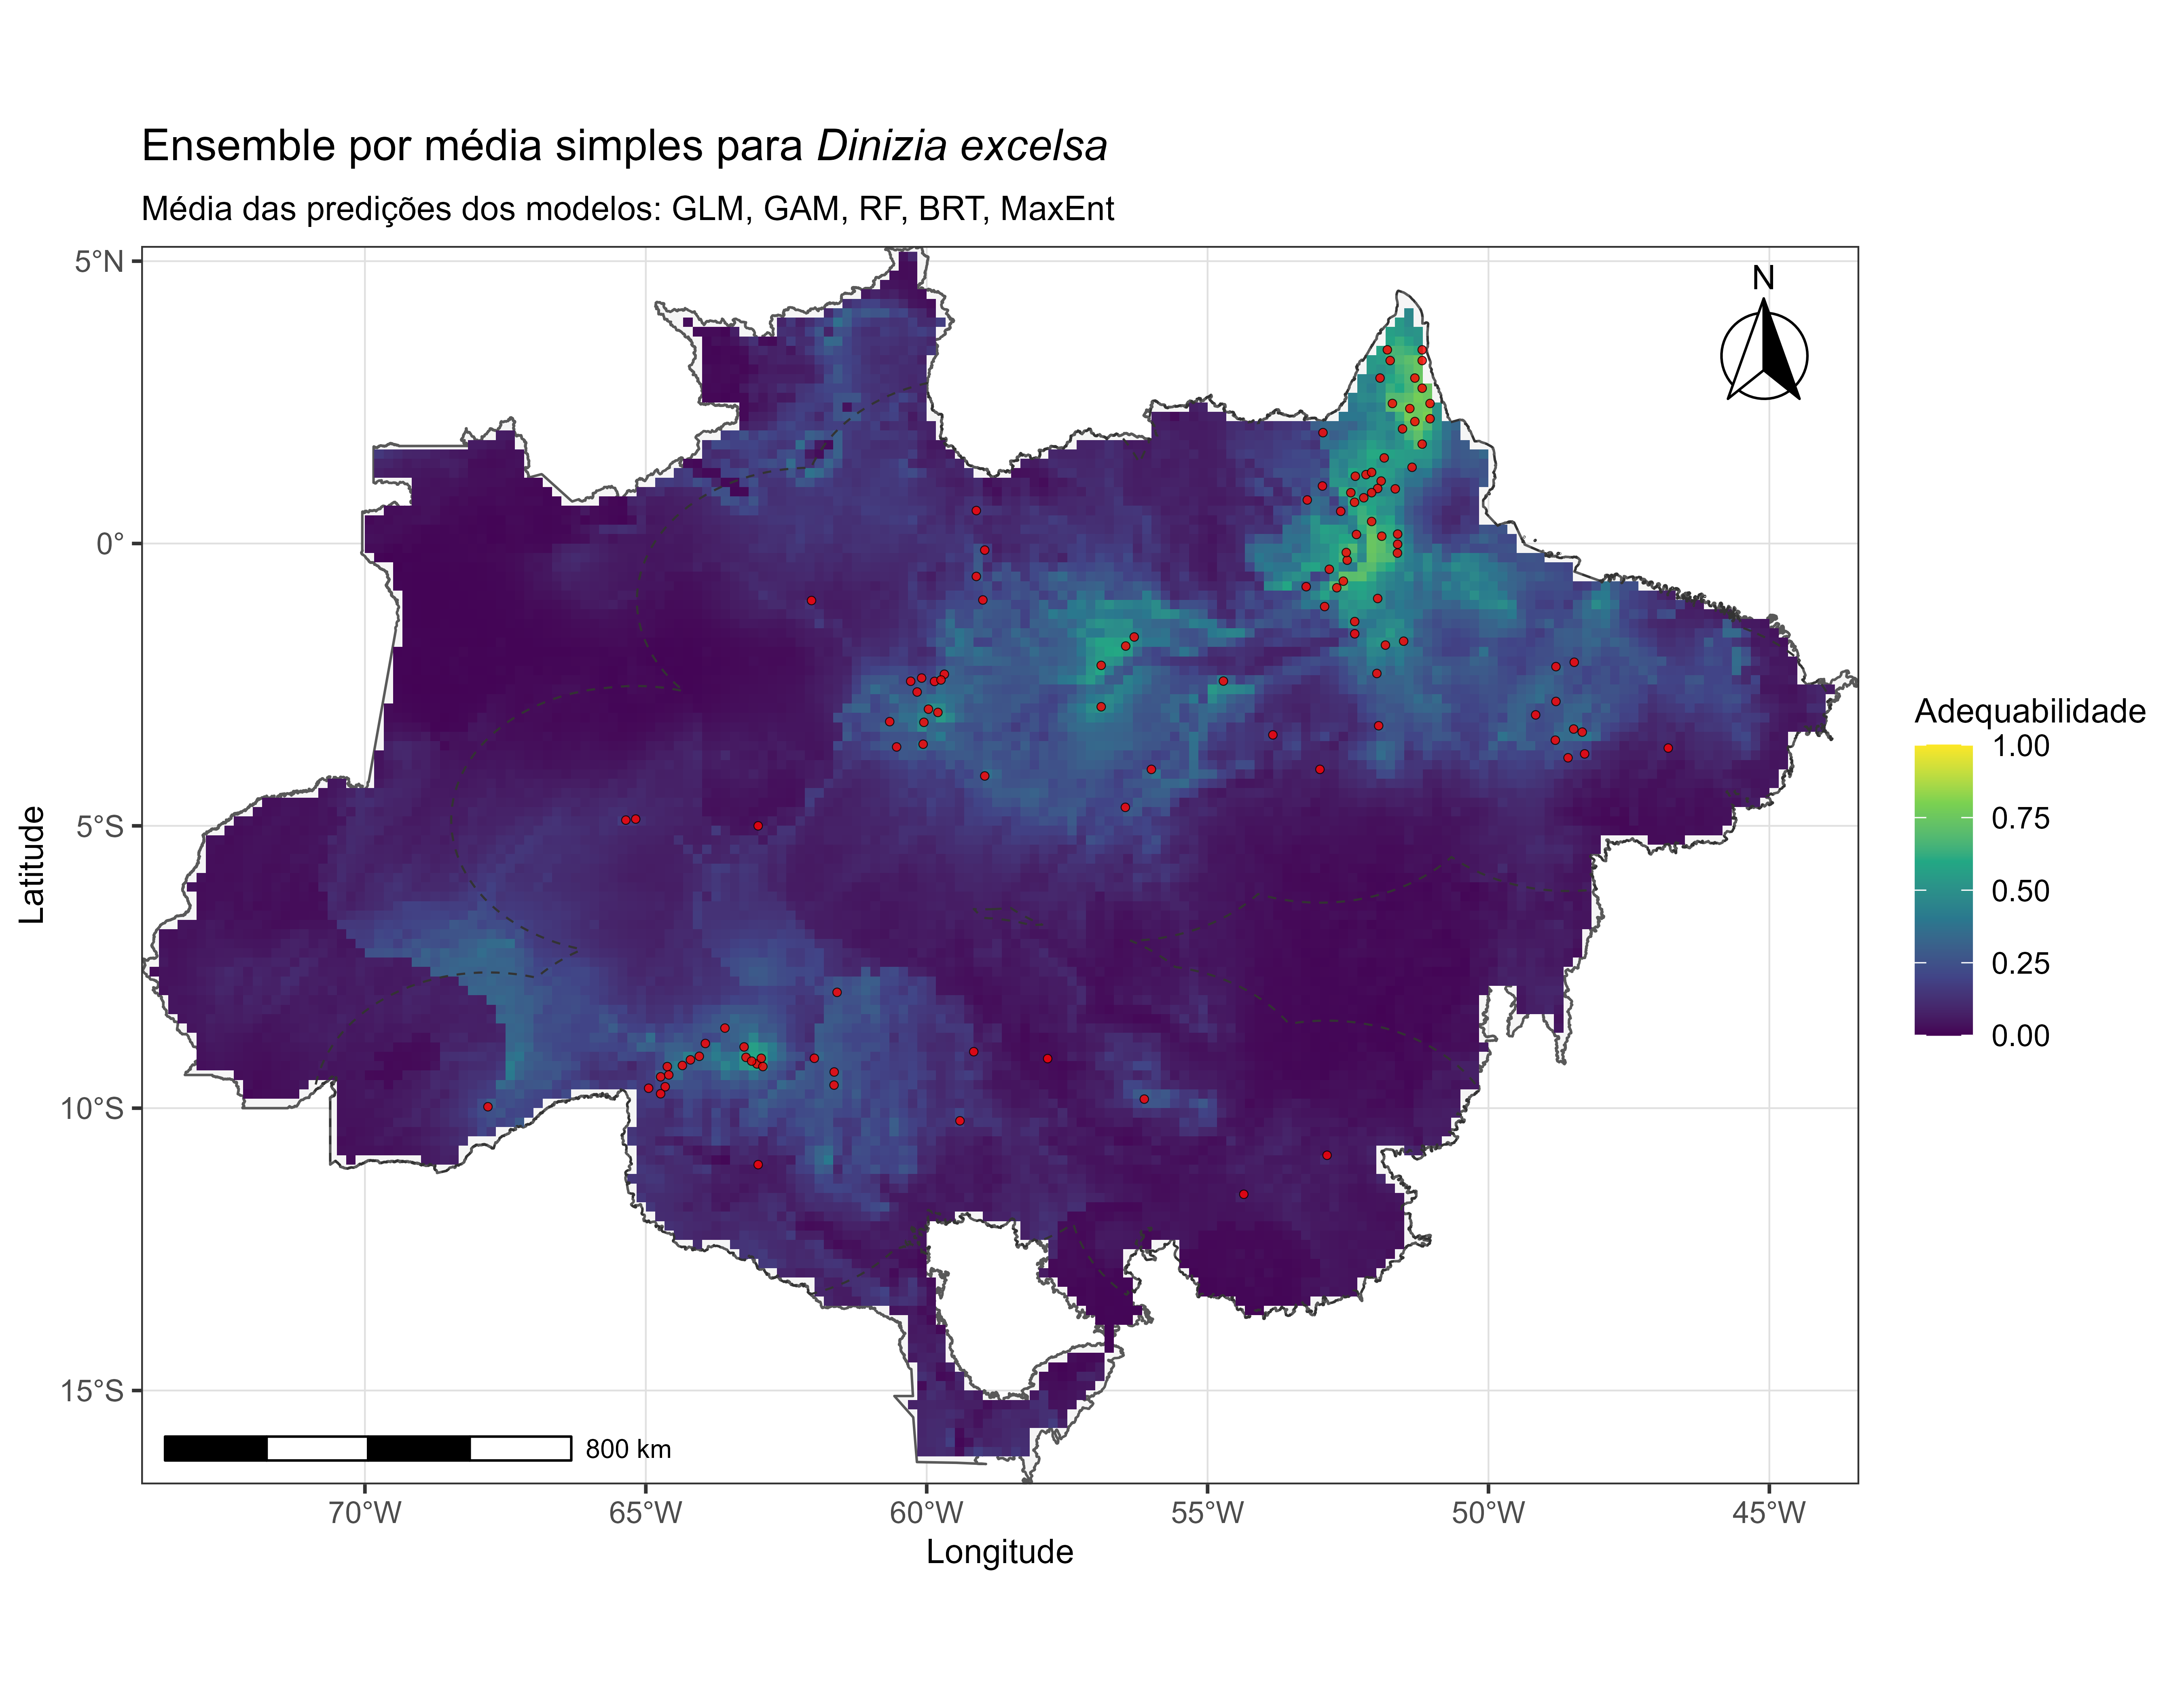
\includegraphics[width=0.88\textwidth]{figuras/unidade11/unidade11_ensemble_media_simples.png}
	\caption{Mapa ensemble por média simples das predições de GLM, GAM, Random Forest, BRT e Maxent para \textit{Dinizia excelsa}.}
	\label{fig:unidade11_ensemble_media}
\end{figure}

\section{Ensemble ponderado por desempenho}

O ensemble ponderado utiliza métricas de avaliação para atribuir maior peso aos modelos com melhor desempenho. Nesta unidade, usamos AUC de teste como critério principal, mas o mesmo procedimento pode ser adaptado para TSS, Boyce Index ou métricas compostas.

\rscriptfile{scripts/unidade11/04_ensemble_ponderado.R}

\begin{figure}[H]
	\centering
	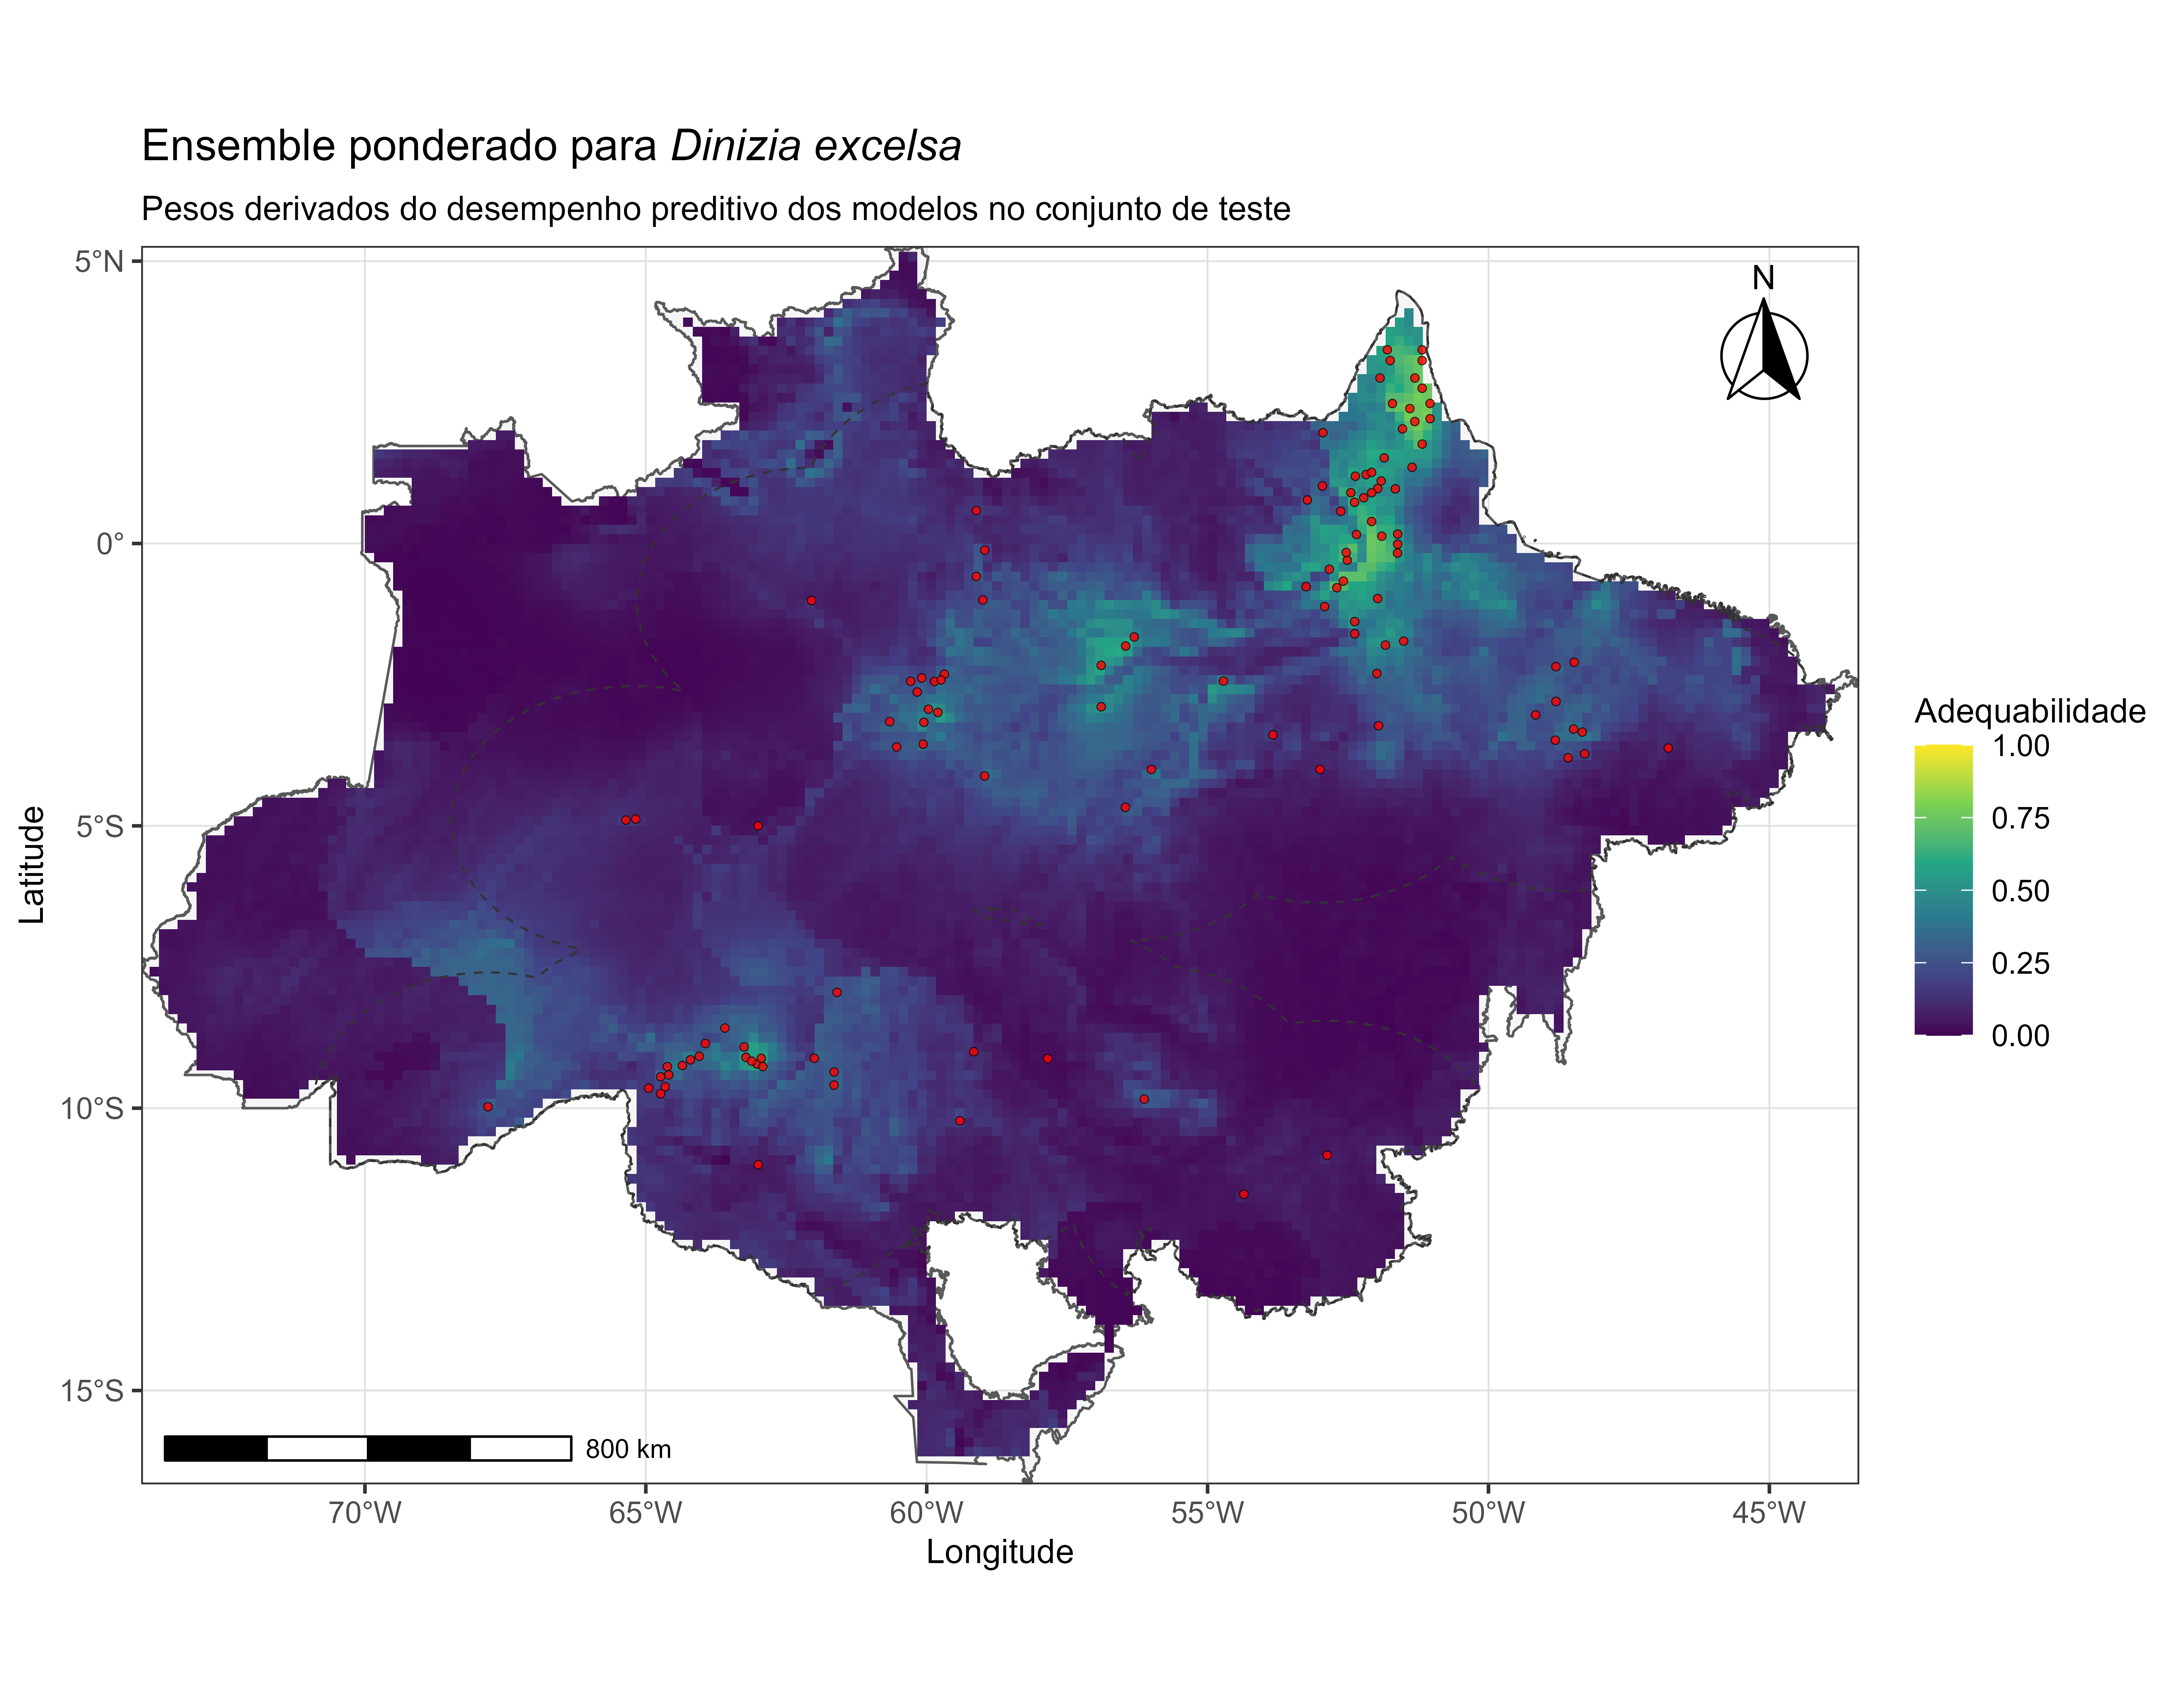
\includegraphics[width=0.88\textwidth]{figuras/unidade11/unidade11_ensemble_ponderado.png}
	\caption{Mapa ensemble ponderado por desempenho preditivo para \textit{Dinizia excelsa}.}
	\label{fig:unidade11_ensemble_ponderado}
\end{figure}

\section{Consenso binário}

O consenso binário converte cada mapa contínuo em presença-ausência usando limiares definidos por TSS. O mapa final representa a proporção de modelos que classificam cada célula como adequada.

\rscriptfile{scripts/unidade11/05_consenso_binario.R}

\begin{figure}[H]
	\centering
	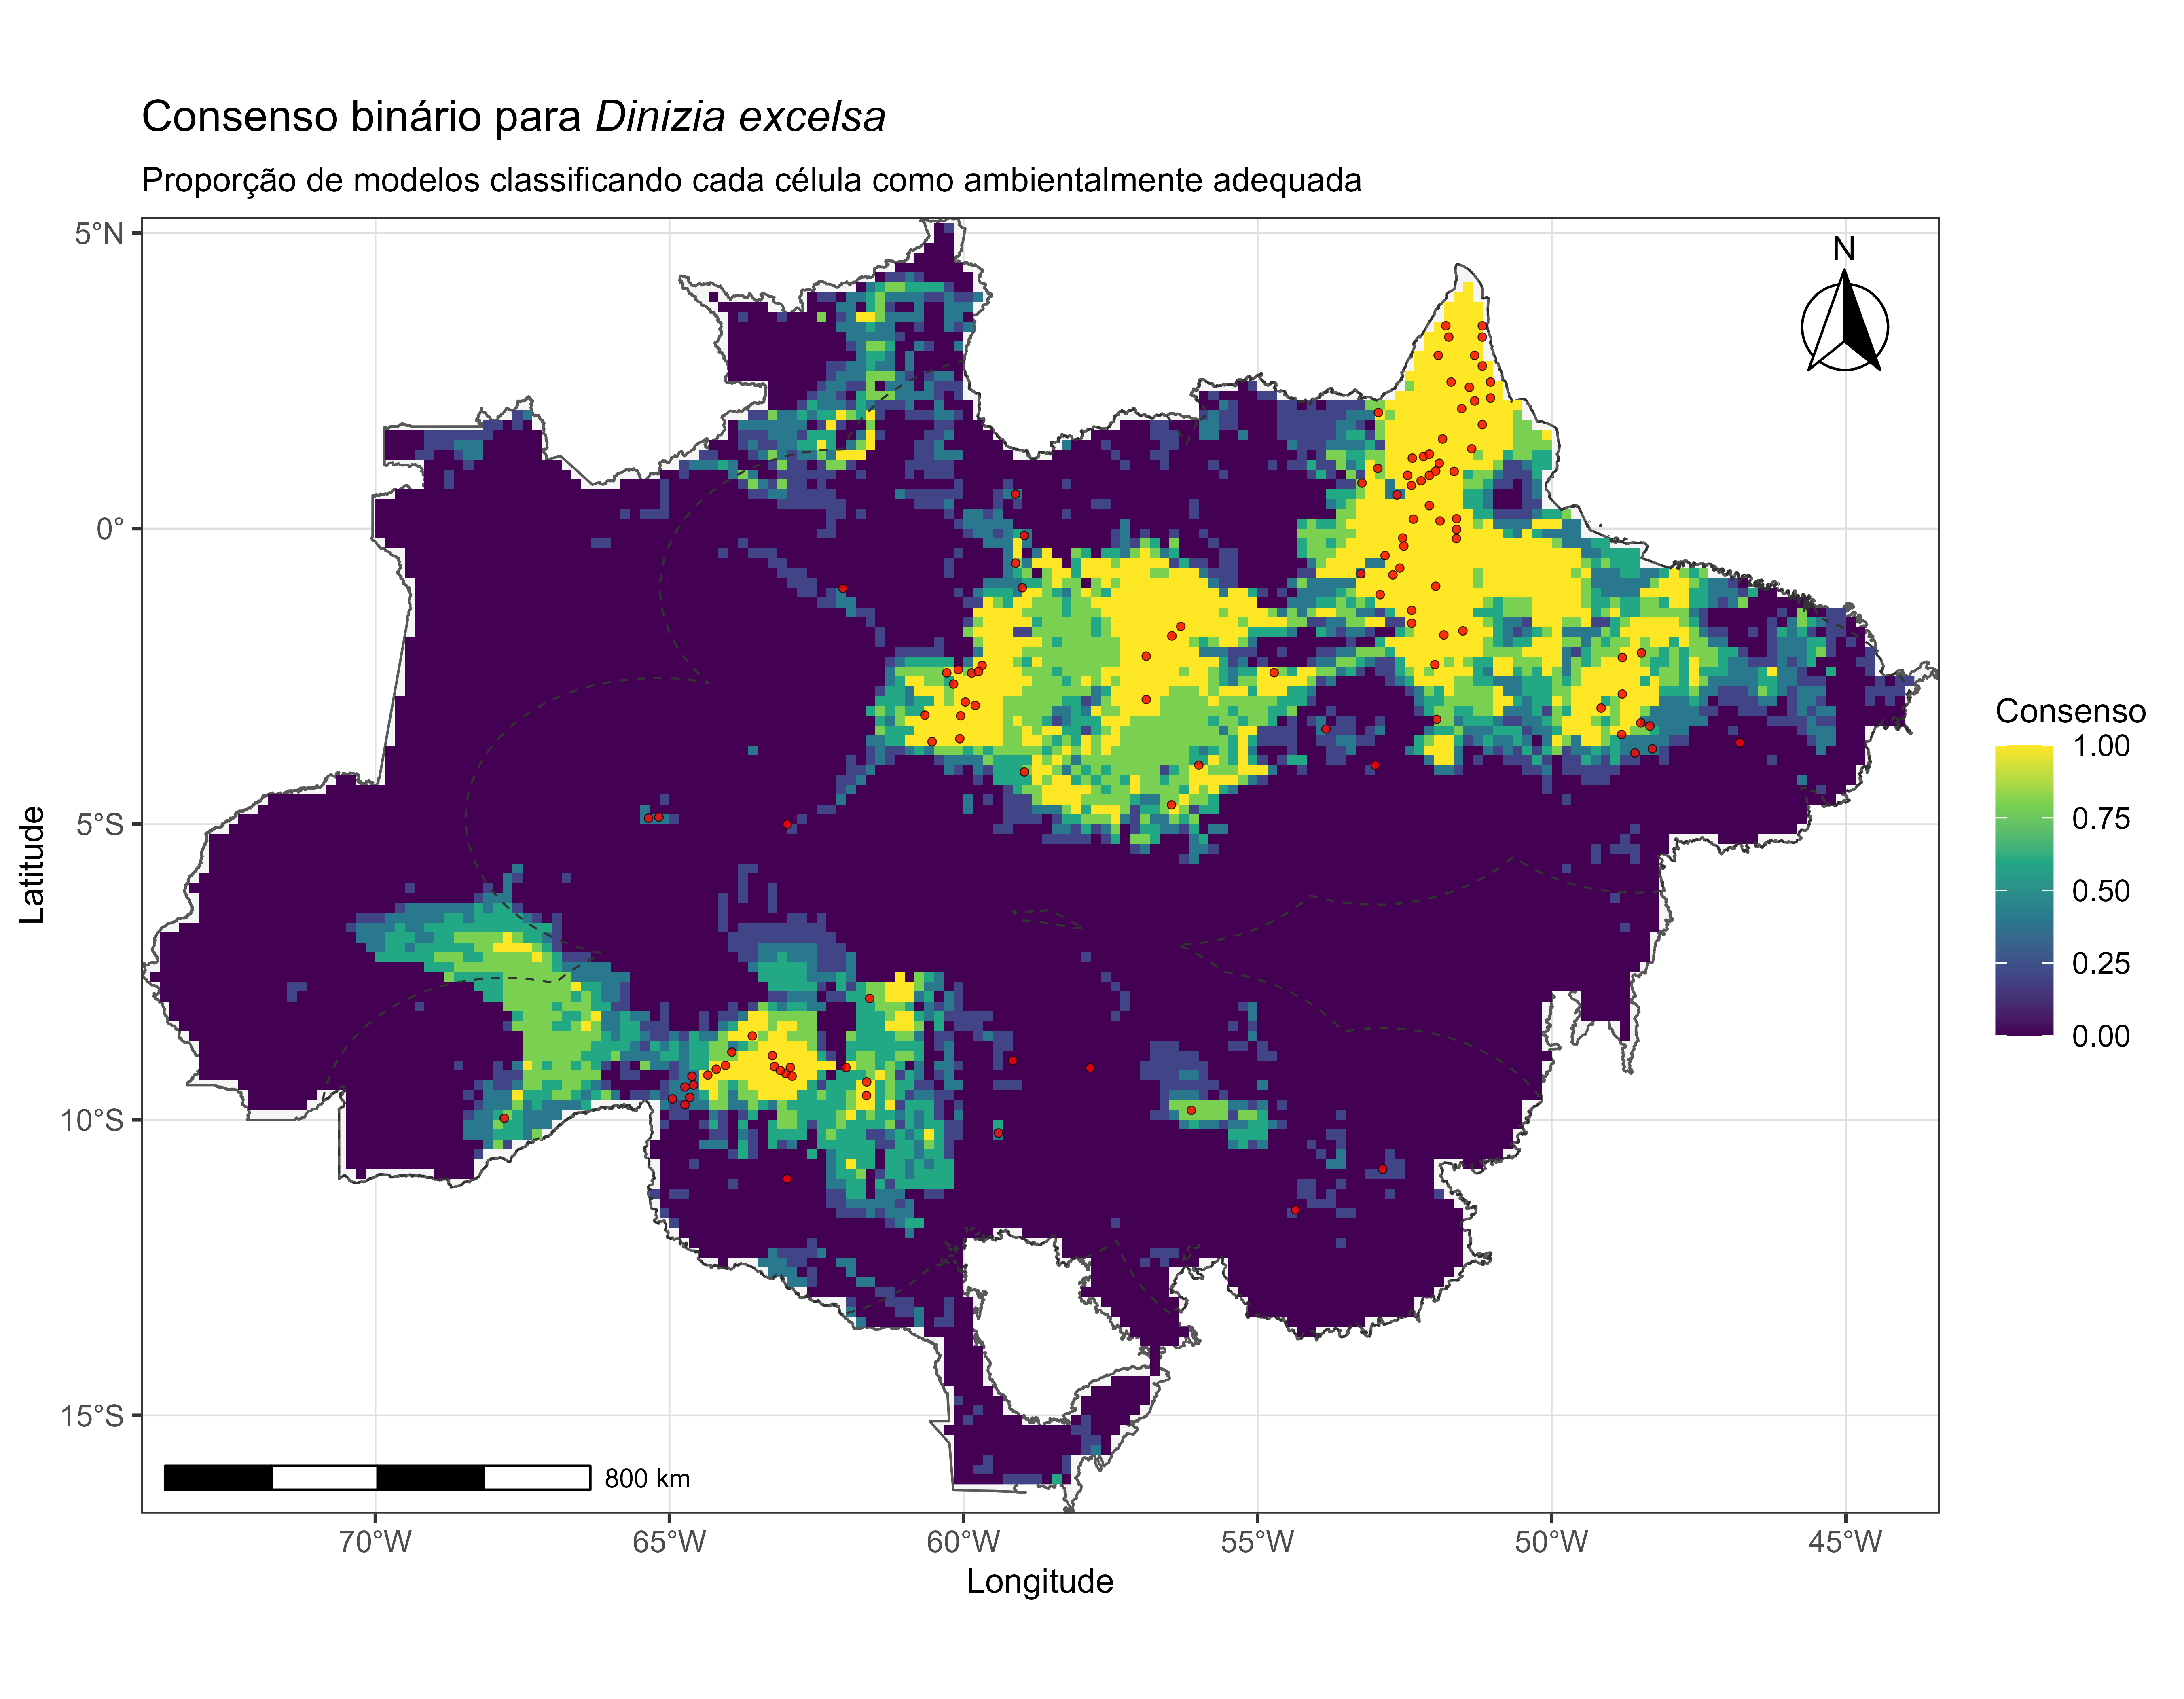
\includegraphics[width=0.88\textwidth]{figuras/unidade11/unidade11_consenso_binario.png}
	\caption{Consenso binário entre os modelos. Valores próximos de 1 indicam alta concordância entre modelos quanto à adequabilidade ambiental.}
	\label{fig:unidade11_consenso_binario}
\end{figure}

\section{Incerteza entre algoritmos}

A variação entre modelos pode ser usada como uma medida de incerteza algorítmica. Regiões com alta adequabilidade média e baixa incerteza são mais robustas; regiões com alta divergência entre modelos exigem interpretação cautelosa.

\rscriptfile{scripts/unidade11/06_incerteza_algoritmica.R}

\begin{figure}[H]
	\centering
	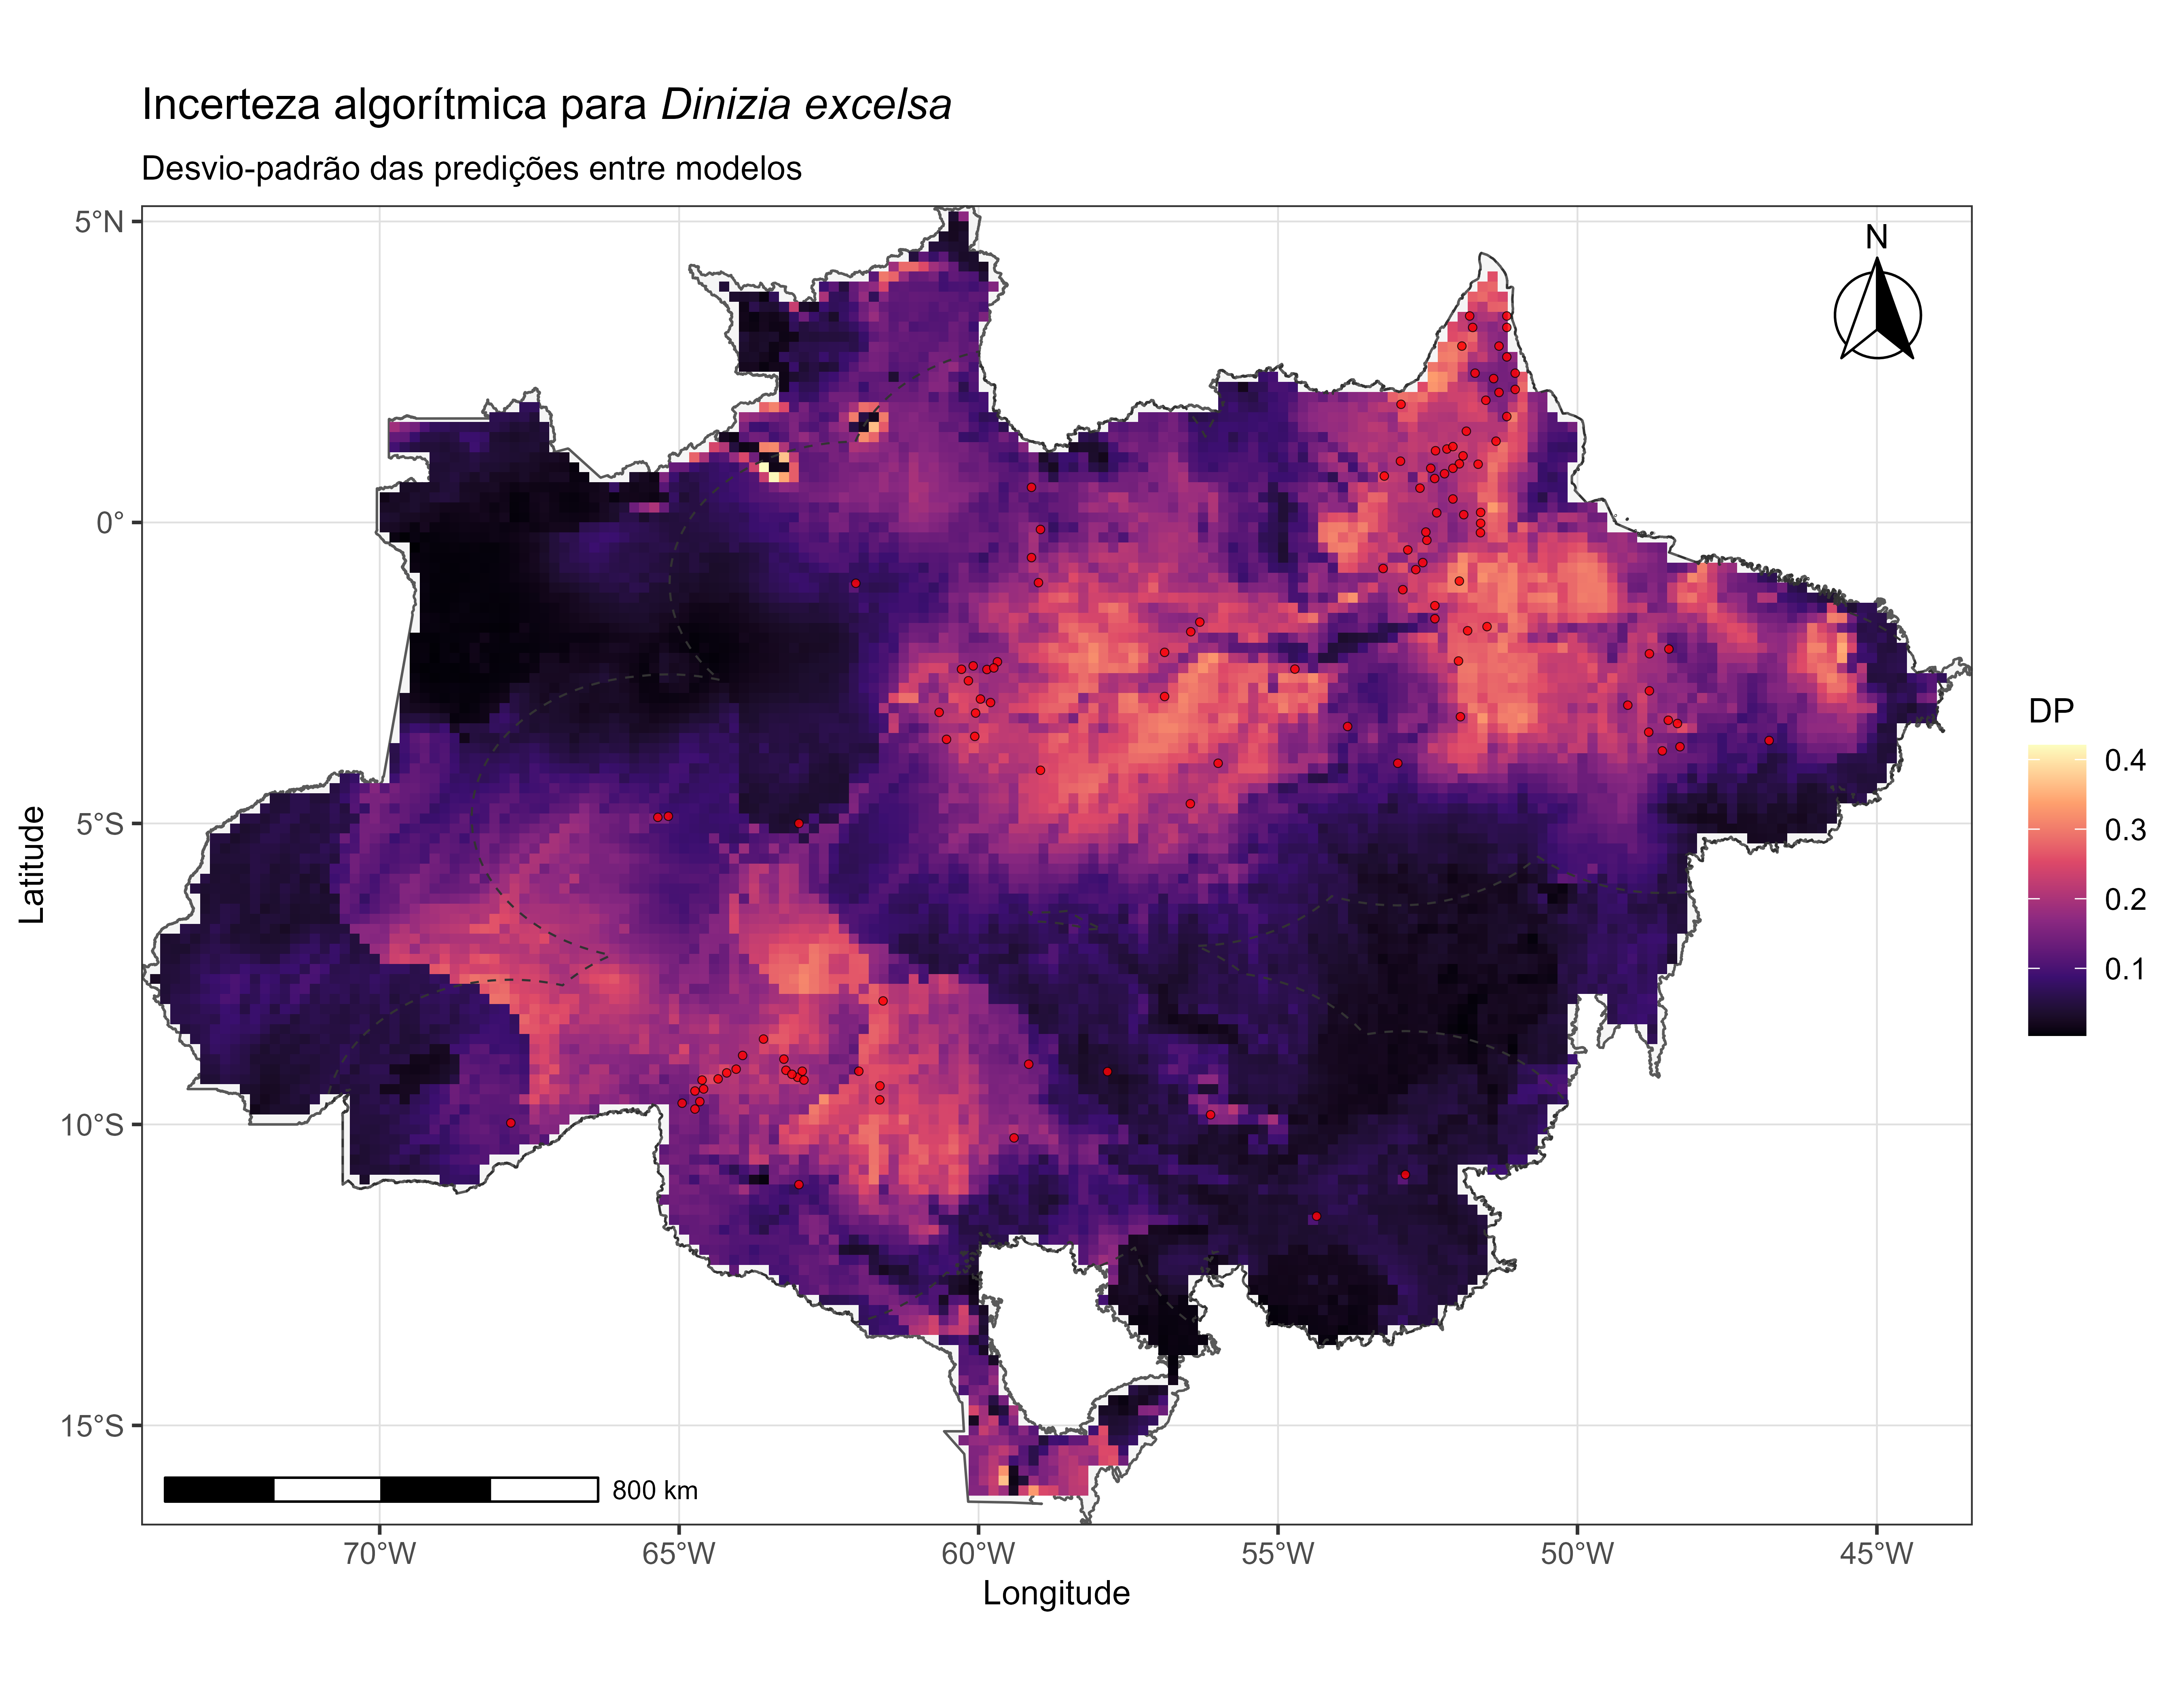
\includegraphics[width=0.88\textwidth]{figuras/unidade11/unidade11_incerteza_algoritmica.png}
	\caption{Incerteza algorítmica estimada pelo desvio-padrão das predições entre modelos.}
	\label{fig:unidade11_incerteza_algoritmica}
\end{figure}

\section{Comparação integrada}

\rscriptfile{scripts/unidade11/07_comparacao_ensemble_modelos.R}

\begin{figure}[H]
	\centering
	\includegraphics[width=0.98\textwidth]{figuras/unidade11/unidade11_comparacao_ensemble.png}
	\caption{Comparação entre modelos individuais, ensemble médio, ensemble ponderado, consenso binário e incerteza algorítmica.}
	\label{fig:unidade11_comparacao_ensemble}
\end{figure}

\section{Pipeline completo}

\rscriptfile{scripts/unidade11/08_pipeline_ensemble.R}

\section{Síntese da unidade}

A modelagem ensemble permite sintetizar diferentes algoritmos em um produto integrado de adequabilidade ambiental. Para \textit{Dinizia excelsa}, o ensemble combina modelos estatísticos interpretáveis e algoritmos flexíveis, oferecendo uma visão mais robusta da distribuição potencial atual dentro da área acessível \(M\).

\begin{conceito}[title={\faBook\quad Mensagem central}]
	O ensemble não substitui a avaliação crítica dos modelos individuais. Ele deve ser interpretado junto com métricas de desempenho, curvas de resposta, coerência ecológica e mapas de incerteza.
\end{conceito}

\section{Exercícios de fixação}

\begin{enumerate}
	\item Explique por que ensembles são usados em SDM.
	\item Diferencie média simples, média ponderada e consenso binário.
	\item Por que modelos ruins não devem ser incluídos no ensemble?
	\item Como a incerteza algorítmica pode ser mapeada?
	\item Por que o ensemble ponderado depende da escolha da métrica?
	\item Como interpretar áreas com alta adequabilidade e alta incerteza?
	\item Explique como o ensemble será útil nas projeções climáticas futuras.
\end{enumerate}

% ============================================================
% UNIDADE 12
% ============================================================

